\begin{figure}[htbp]
    \centering
    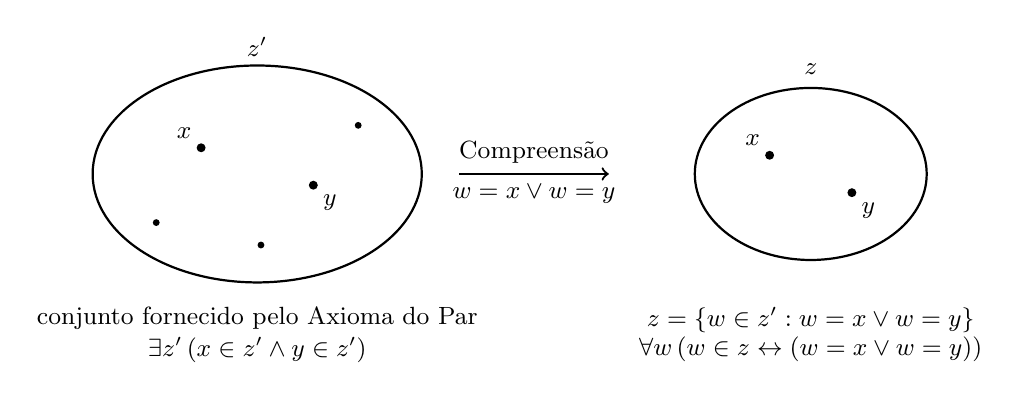
\begin{tikzpicture}[scale=0.95, every node/.style={font=\small}]
        % Conjunto z'
        \draw[thick] (0,0) ellipse (2.2 and 1.45);
        \node at (0,1.7) {$z'$};

        \fill (-0.75,0.35) circle (1.7pt);
        \node[above left] at (-0.75,0.35) {$x$};

        \fill (0.75,-0.15) circle (1.7pt);
        \node[below right] at (0.75,-0.15) {$y$};

        \fill (-1.35,-0.65) circle (1.3pt);
        \fill (1.35,0.65) circle (1.3pt);
        \fill (0.05,-0.95) circle (1.3pt);

        \node[below,align=center] at (0,-1.65)
            {conjunto fornecido pelo Axioma do Par};
        \node[below,align=center] at (0,-2.05)
            {$\exists z'\,(x\in z'\land y\in z')$};

        % Seta de compreensão
        \draw[->,thick] (2.7,0) -- (4.7,0)
            node[midway,above,align=center] {Compreens\~ao}
            node[midway,below,align=center] {$w=x\lor w=y$};

        % Conjunto z
        \draw[thick] (7.4,0) ellipse (1.55 and 1.15);
        \node at (7.4,1.4) {$z$};

        \fill (6.85,0.25) circle (1.7pt);
        \node[above left] at (6.85,0.25) {$x$};

        \fill (7.95,-0.25) circle (1.7pt);
        \node[below right] at (7.95,-0.25) {$y$};

        \node[below,align=center] at (7.4,-1.65)
            {$z=\{w\in z' : w=x\lor w=y\}$};
        \node[below,align=center] at (7.4,-2.05)
            {$\forall w\,(w\in z \leftrightarrow (w=x\lor w=y))$};
    \end{tikzpicture}

    \caption{O Axioma do Par fornece um conjunto $z'$ que possui $x$ e $y$ como elementos.
    Aplicando o Esquema da Compreensão a $z'$ obtém-se o subconjunto $z$ cujos únicos elementos são $x$ e $y$.}
    \label{fig:compreensaoDoPar}
\end{figure}